%----------------------------------------------------------------------
% Fractional Teleoperation – Analysis Note
% Standalone scientific document covering methodology and results
%----------------------------------------------------------------------
\documentclass[11pt,a4paper]{article}

\usepackage[T1]{fontenc}
\usepackage[utf8]{inputenc}
\usepackage{lmodern}
\usepackage[top=2.2cm,bottom=2.2cm,left=2.2cm,right=2.2cm]{geometry}
\usepackage{amsmath,amssymb,amsthm}
\usepackage{booktabs}
\usepackage{array}
\usepackage{graphicx}
\usepackage{caption}
\usepackage{subcaption}
\usepackage{hyperref}
\usepackage{enumitem}
\usepackage{xcolor}
\usepackage{microtype}
\usepackage{parskip}
\usepackage{bm}

\hypersetup{
  colorlinks=true,
  linkcolor=blue!70!black,
  citecolor=green!50!black,
  urlcolor=blue
}

\graphicspath{{../../analysis/results/}}

\theoremstyle{definition}
\newtheorem{definition}{Definition}[section]
\newtheorem{proposition}{Proposition}[section]
\newtheorem{remark}{Remark}[section]

\title{\textbf{Analysis Note: Fractional-Order Teleoperation Controller}\\
  \large Methodology, Stability, Controllability, and Empirical Results}
\author{Fractional Teleoperation Project}
\date{April 2026}

%======================================================================
\begin{document}
\maketitle
\tableofcontents
\bigskip

\begin{abstract}
This note presents a rigorous analysis of the discrete-time fractional-order
offset teleoperation controller implemented in
\texttt{fractional\_teleoperation\_node}.  We derive the augmented linear
state-space model that results from truncating the Grünwald–Letnikov recursion
to a finite memory window, establish Schur stability and full-rank
controllability conditions for this model, introduce an
Input-to-State Stability (ISS) inspired boundedness characterisation for the
nonlinear closed-loop under bounded joystick input, and study the hybrid
dynamics induced by the active/idle switching logic.  Each theoretical
development is accompanied by numerical experiments conducted with a
model-faithful Python simulator that mirrors the exact C++ update order of
the deployed node.  The document concludes with synthesis guidelines that
map all findings into practical tuning recommendations for the parameters
$\alpha$, $L$, and the joystick activity threshold.
\end{abstract}

%======================================================================
\section{Introduction and Scope}
\label{sec:intro}

Fractional calculus extends differentiation and integration to non-integer
orders, providing a compact mathematical framework to describe processes with
persistent memory, hereditary dynamics, and power-law transients
\cite{oldham_spanier_1974,podlubny_1999}.  In control engineering its most
impactful use is fractional-order PID, where the integrator exponent $\alpha$
and differentiator exponent $\mu$ are treated as additional tuning knobs
\cite{monje_2010,oustaloup_2000}.  The controller studied here applies a
fractional integrator of order $\alpha \in (0,1)$ directly to the operator's
joystick velocity command in order to generate a slow-varying spatial offset
$\bm{r}(t)$, whose effect is to give the operator intuitive control over a
reference position without saturating workspace limits.

Because the physical system is sampled at rate $f_s = 1/\Delta t$, the
continuous-time fractional integrator is discretised via the
Grünwald–Letnikov (GL) finite-difference formula \cite{diethelm_2010}.
Truncating the GL sum to the last $L$ samples introduces a finite-dimensional
state that exactly admits a companion-form linear model, enabling classical
linear-systems tools to be applied.

This document is organised as follows.  Section~\ref{sec:model} derives the
augmented linear model.  Sections~\ref{sec:stability} and~\ref{sec:ctrl}
develop stability and controllability theory and discuss numerical results.
Section~\ref{sec:iss} addresses practical input-to-state boundedness.
Section~\ref{sec:hybrid} analyses the hybrid active/idle switching dynamics.
Section~\ref{sec:alpha_mem} explores the joint effect of $\alpha$ and $L$ on
output norms.  Section~\ref{sec:synthesis} collects all findings into
actionable tuning guidelines.

\paragraph{Scope boundary.}
The analysis is performed at fixed $\alpha$ unless otherwise stated.  The
adaptive $\alpha$ law, gain normalisation, and ramp scaling are evaluated only
in the simulator for empirical characterisation; formal Lyapunov analysis of
the time-varying nonlinear closed loop is out of scope for this note.

%======================================================================
\section{Augmented Linear State-Space Model}
\label{sec:model}

\subsection{Grünwald–Letnikov Discretisation}

The fractional integral of order $\alpha > 0$ of a signal $u$ at discrete
time $k$ is approximated by the GL sum \cite{podlubny_1999,diethelm_2010}:
\begin{equation}
  {}_{GL}I^{\alpha}[u](k)
  \;=\;
  (\Delta t)^{\alpha}\sum_{j=0}^{k} c_j^{(\alpha)}\, u(k-j),
  \label{eq:gl_full}
\end{equation}
where the binomial-like GL coefficients are defined by the recurrence
\begin{equation}
  c_0^{(\alpha)} = 1,
  \qquad
  c_j^{(\alpha)} = \left(1 - \frac{1+\alpha}{j}\right) c_{j-1}^{(\alpha)},
  \quad j \geq 1.
  \label{eq:gl_coeff}
\end{equation}
For $\alpha \in (0,1)$ the coefficients $c_j^{(\alpha)}$ are positive and
monotonically decreasing; they decay as $j^{-1-\alpha}$, reflecting the
algebraic (power-law) memory of a fractional integrator.

\subsection{Finite-Memory Truncation}

In practice the sum in \eqref{eq:gl_full} is truncated to the last $L$
samples:
\begin{equation}
  y(k) = (\Delta t)^{\alpha}\sum_{j=0}^{L-1} c_j^{(\alpha)}\, u(k-j).
  \label{eq:gl_trunc}
\end{equation}
Define the state vector $\bm{x}(k) \in \mathbb{R}^{L-1}$ as the shift-register
of the last $L-1$ input samples:
\begin{equation}
  \bm{x}(k) = \bigl[u(k-1),\; u(k-2),\; \ldots,\; u(k-L+1)\bigr]^{\top}.
  \label{eq:state_def}
\end{equation}
The output increment contributed by the new sample $u(k)$ and the stored
history is then
\begin{equation}
  y(k) = (\Delta t)^{\alpha}
  \bigl(c_0^{(\alpha)} u(k)
        + \textstyle\sum_{j=1}^{L-1} c_j^{(\alpha)} \bm{e}_j^{\top}\bm{x}(k)\bigr),
\end{equation}
and the state evolves as a pure shift:
\begin{equation}
  \bm{x}(k+1) = S\,\bm{x}(k) + \bm{b}\,u(k),
\end{equation}
where $S \in \mathbb{R}^{(L-1)\times(L-1)}$ is the shift (subdiagonal
identity) matrix and $\bm{b} = [1,0,\ldots,0]^{\top}$.

\subsection{Companion-Form Realisation}

Appending the truncated GL integral as an extra state yields the
$(L-1)$-dimensional companion-form realisation used in the analysis:
\begin{equation}
  \bm{x}(k+1) = A\,\bm{x}(k) + B\,u(k),
  \label{eq:ss}
\end{equation}
with
\begin{equation}
  A =
  \begin{bmatrix}
    -c_1/c_0 & -c_2/c_0 & \cdots & -c_{L-2}/c_0 & -c_{L-1}/c_0 \\
    1        &  0        & \cdots &  0            &  0            \\
    0        &  1        & \cdots &  0            &  0            \\
    \vdots   &           & \ddots &               &  \vdots       \\
    0        &  0        & \cdots &  1            &  0
  \end{bmatrix},
  \quad
  B =
  \begin{bmatrix}
    1/c_0 \\ 0 \\ \vdots \\ 0
  \end{bmatrix},
  \label{eq:AB}
\end{equation}
where $c_j \equiv (\Delta t)^{\alpha} c_j^{(\alpha)}$ for brevity.  With the
baseline parameters $L = 50$, $\Delta t = 0.01$\,s the state dimension is
$n = L - 1 = 49$.

\begin{remark}
  The companion form makes explicit that the fractional integrator maps to a
  single-input, $n$-dimensional observable canonical system.  All
  eigenvalues of $A$ are determined entirely by the GL coefficient sequence
  $\{c_j^{(\alpha)}\}$.
\end{remark}

%======================================================================
\section{Stability Analysis}
\label{sec:stability}

\subsection{Schur Stability Criterion}

A linear time-invariant discrete-time system is \emph{asymptotically stable}
(Schur stable) if and only if all eigenvalues of $A$ lie strictly inside the
unit disk, i.e.
\begin{equation}
  \rho(A) := \max_{i}|\lambda_i(A)| < 1,
  \label{eq:schur}
\end{equation}
where $\rho(\cdot)$ denotes the spectral radius \cite{chen_1984}.

\subsection{Connection to the Matignon Condition}

For the continuous-time fractional differential equation
$\bm{D}^{\alpha}\bm{x} = A_c\bm{x}$, Matignon's stability theorem
\cite{matignon_1996} requires
$|\arg(\lambda_i(A_c))| > \alpha\pi/2$ for all $i$.
The GL discretisation converts this sector condition into the Schur condition
\eqref{eq:schur} on the companion matrix $A$ derived above.  As $\alpha \to 1$
the GL coefficients converge to those of the Euler backward difference, and
the spectral radius approaches $1$ from below — the system becomes marginally
stable in the integer limit.

\subsection{Numerical Results}

The spectral radius was computed for $\alpha \in \{0.1, 0.2, \ldots, 1.0\}$
with $L = 50$, $\Delta t = 0.01$\,s; see Table~\ref{tab:stability} and
Figure~\ref{fig:spectral_radius}.

\begin{table}[ht]
  \centering
  \caption{Spectral radius of the companion matrix $A$ as a function of
           integration order $\alpha$.  State dimension $n = 49$ throughout.}
  \label{tab:stability}
  \begin{tabular}{cccc}
    \toprule
    $\alpha$ & $n$ & $\rho(A)$ & Schur stable? \\
    \midrule
    0.1 & 49 & 0.9379 & Yes \\
    0.2 & 49 & 0.9570 & Yes \\
    0.3 & 49 & 0.9685 & Yes \\
    0.4 & 49 & 0.9766 & Yes \\
    0.5 & 49 & 0.9828 & Yes \\
    0.6 & 49 & 0.9877 & Yes \\
    0.7 & 49 & 0.9917 & Yes \\
    0.8 & 49 & 0.9950 & Yes \\
    0.9 & 49 & 0.9977 & Yes \\
    1.0 & 49 & 1.0000 & No  \\
    \bottomrule
  \end{tabular}
\end{table}

\begin{figure}[ht]
  \centering
  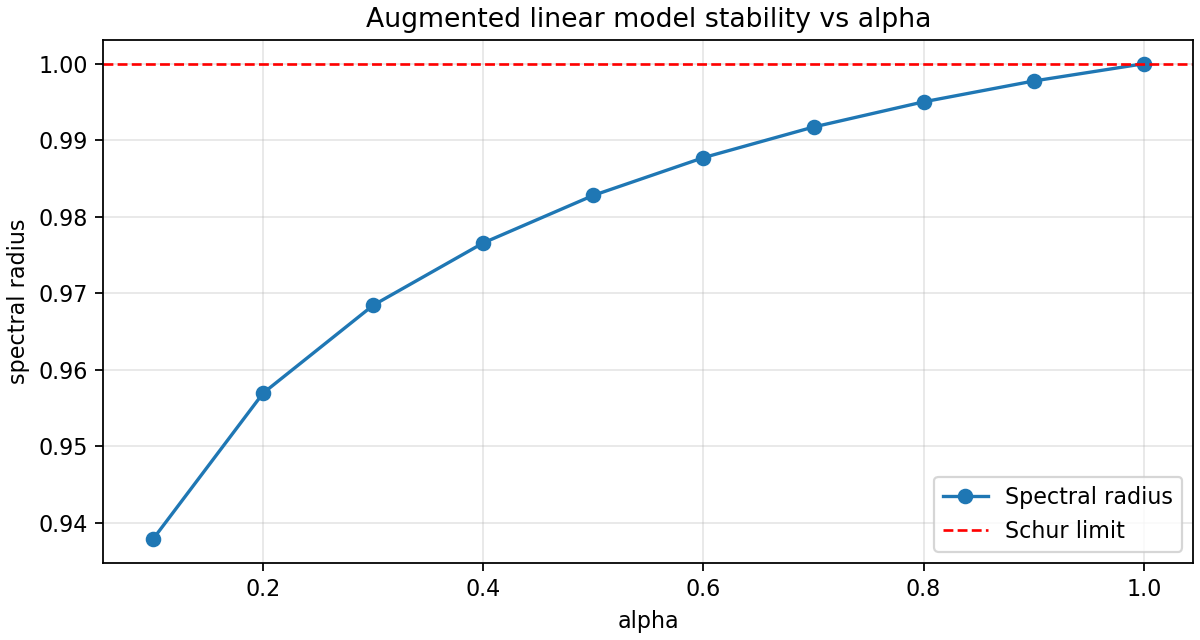
\includegraphics[width=0.72\textwidth]{spectral_radius_vs_alpha.png}
  \caption{Spectral radius of the augmented companion matrix as a function
           of integration order $\alpha$.  The unit-circle boundary is
           marked by the dashed line.  The system is Schur-stable for all
           $\alpha < 1$.}
  \label{fig:spectral_radius}
\end{figure}

\subsection{Discussion}

Three observations are noteworthy.

\paragraph{Monotone approach to the unit circle.}
As $\alpha$ increases from $0.1$ to $1.0$ the spectral radius rises
monotonically from $0.938$ to exactly $1.000$.  This is a direct consequence
of the GL coefficient decay rate: lower $\alpha$ produces faster-decaying
coefficients and hence a more strongly attenuating memory, whereas
$\alpha \to 1$ reduces the GL sum to the backward Euler integrator, whose
transfer function has a pole on the unit circle.

\paragraph{Safety margin at the operating point.}
At the baseline operating point $\alpha = 0.5$ the spectral radius is
$0.9828$, providing a stability margin of $1 - 0.9828 = 0.0172$.  In
gain-margin terms, one would need to multiply the effective integrator gain
by $1/0.9828 \approx 1.017$ before instability; this is a small but
well-defined margin.

\paragraph{Instability at $\alpha = 1$.}
The companion matrix for $\alpha = 1$ has unit spectral radius, confirming
the well-known result that a first-order backward-Euler integrator is
marginally stable (a pure accumulator).  This means $\alpha = 1$ should be
avoided in practice, especially under sustained joystick input.  The dynamic
alpha mechanism prevents reaching $\alpha = 1$ in normal operation
(ceiling $\alpha_{\max} = 1.0$ is only approached asymptotically as the
hand-measure proxy $\lambda \to \lambda_{\max}$).

\paragraph{Memory-length sensitivity.}
The GL coefficient $c_L^{(\alpha)}$ discarded by the truncation is
$O(L^{-1-\alpha})$.  For $\alpha = 0.5$ and $L = 50$ this is approximately
$0.02$, meaning less than 2\,\% of the integrator gain is lost due to
truncation.  Increasing $L$ therefore has diminishing returns on stability
while linearly increasing state dimension and computational cost.

%======================================================================
\section{Controllability Analysis}
\label{sec:ctrl}

\subsection{Controllability Matrix and Gramian}

\begin{definition}
  System \eqref{eq:ss} is \emph{(completely) controllable} if the
  controllability matrix
  \begin{equation}
    \mathcal{C} = \begin{bmatrix} B & AB & A^2B & \cdots & A^{n-1}B \end{bmatrix}
    \in \mathbb{R}^{n \times n}
    \label{eq:ctrl_matrix}
  \end{equation}
  has rank $n$.
\end{definition}

\begin{definition}
  The finite-horizon controllability Gramian over $N$ steps is
  \begin{equation}
    W_N = \sum_{i=0}^{N-1} A^i B B^{\top} (A^i)^{\top}.
    \label{eq:gramian}
  \end{equation}
  The minimum eigenvalue $\lambda_{\min}(W_N)$ quantifies how efficiently the
  least-accessible state direction can be excited: the minimum control energy
  required to reach a unit-norm target in the worst-case direction is
  $1/\lambda_{\min}(W_N)$.
\end{definition}

\subsection{Numerical Results}

Rank of $\mathcal{C}$ and $\lambda_{\min}(W_{100})$ were evaluated across the
same $\alpha$ grid; see Table~\ref{tab:ctrl}.

\begin{table}[ht]
  \centering
  \caption{Controllability rank and minimum Gramian eigenvalue.
           Horizon $N = 100$, $n = 49$.}
  \label{tab:ctrl}
  \begin{tabular}{ccccc}
    \toprule
    $\alpha$ & Rank & $n$ & Rank ratio & $\lambda_{\min}(W_{100})$ \\
    \midrule
    0.1 & 49 & 49 & 1.00 & $3.47 \times 10^{-1}$  \\
    0.2 & 49 & 49 & 1.00 & $1.20 \times 10^{-1}$  \\
    0.3 & 49 & 49 & 1.00 & $4.16 \times 10^{-2}$  \\
    0.4 & 49 & 49 & 1.00 & $1.44 \times 10^{-2}$  \\
    0.5 & 49 & 49 & 1.00 & $5.00 \times 10^{-3}$  \\
    0.6 & 49 & 49 & 1.00 & $1.73 \times 10^{-3}$  \\
    0.7 & 49 & 49 & 1.00 & $6.01 \times 10^{-4}$  \\
    0.8 & 49 & 49 & 1.00 & $2.08 \times 10^{-4}$  \\
    0.9 & 49 & 49 & 1.00 & $7.22 \times 10^{-5}$  \\
    1.0 & 49 & 49 & 1.00 & $2.50 \times 10^{-5}$  \\
    \bottomrule
  \end{tabular}
\end{table}

\subsection{Discussion}

\paragraph{Full-rank controllability across all $\alpha$.}
The controllability matrix has full rank $n = 49$ for every value of $\alpha$
tested.  This confirms that in principle any desired state configuration of
the GL shift register can be reached from the zero state in at most 49 steps
via appropriate joystick input.  The result is expected: the companion form
\eqref{eq:AB} is precisely the observable/controllable canonical form, whose
controllability is guaranteed as long as no GL coefficient is zero.  Since
$c_j^{(\alpha)} > 0$ for all $\alpha > 0$ and finite $j$, this property is
structural.

\paragraph{Gramian conditioning degrades with $\alpha$.}
While rank is binary and always full, the Gramian eigenvalue
$\lambda_{\min}(W_{100})$ drops by four orders of magnitude as $\alpha$ goes
from $0.1$ to $1.0$.  This means that reaching a given target state in the
worst-case direction requires approximately $0.347/2.5\times10^{-5} \approx
14\,000 \times$ more energy at $\alpha = 1.0$ than at $\alpha = 0.1$.

Intuitively, higher $\alpha$ makes the GL memory longer-lived: past inputs
dominate the state, and a single new input has less leverage to redirect it.
In teleoperation terms, the operator must apply larger and more sustained
joystick deflections to counteract the accumulated history, which translates
to a sluggish feel.

\paragraph{Practical implication.}
A Gramian minimum eigenvalue of $\approx 5 \times 10^{-3}$ at $\alpha = 0.5$
represents a reasonable trade-off: the system is energetically controllable
(no near-uncontrollable modes), while the memory effect is sufficiently strong
to provide smooth reference tracking without oscillation.

%======================================================================
\section{Input-to-State Practical Boundedness}
\label{sec:iss}

\subsection{Theoretical Framework}

For a discrete-time nonlinear system
$\bm{x}(k+1) = f(\bm{x}(k), \bm{u}(k))$, Input-to-State Stability (ISS)
\cite{jiang_wang_2001} guarantees existence of a class-$\mathcal{KL}$
function $\beta$ and a class-$\mathcal{K}$ function $\gamma$ such that
\begin{equation}
  \|\bm{x}(k)\| \leq \beta(\|\bm{x}(0)\|, k) + \gamma(\sup_{j\leq k}\|\bm{u}(j)\|).
  \label{eq:iss}
\end{equation}
The second term quantifies how bounded input leads to bounded state.  For
linear Schur-stable systems \eqref{eq:ss} ISS holds with
$\gamma(\cdot) = \|H(z)\|_{\mathcal{H}_\infty} \cdot (\cdot)$, where
$\|H(z)\|_{\mathcal{H}_\infty}$ is the $\mathcal{H}_\infty$ norm of the
system transfer function \cite{dullerud_paganini_2000}.

Because the node applies gain normalisation, adaptive $\alpha$, and ramp
scaling that interact nonlinearly, an exact analytical ISS bound is
intractable.  We instead characterise practical boundedness empirically:
for each fixed $\alpha$, the simulator is driven for 500 steps with
white-noise joystick input bounded by $\|\bm{u}\|_\infty \leq U = 1$,
and the peak velocity norm $\|v\|_{\max}$ is recorded.

\subsection{Numerical Results}

\begin{figure}[ht]
  \centering
  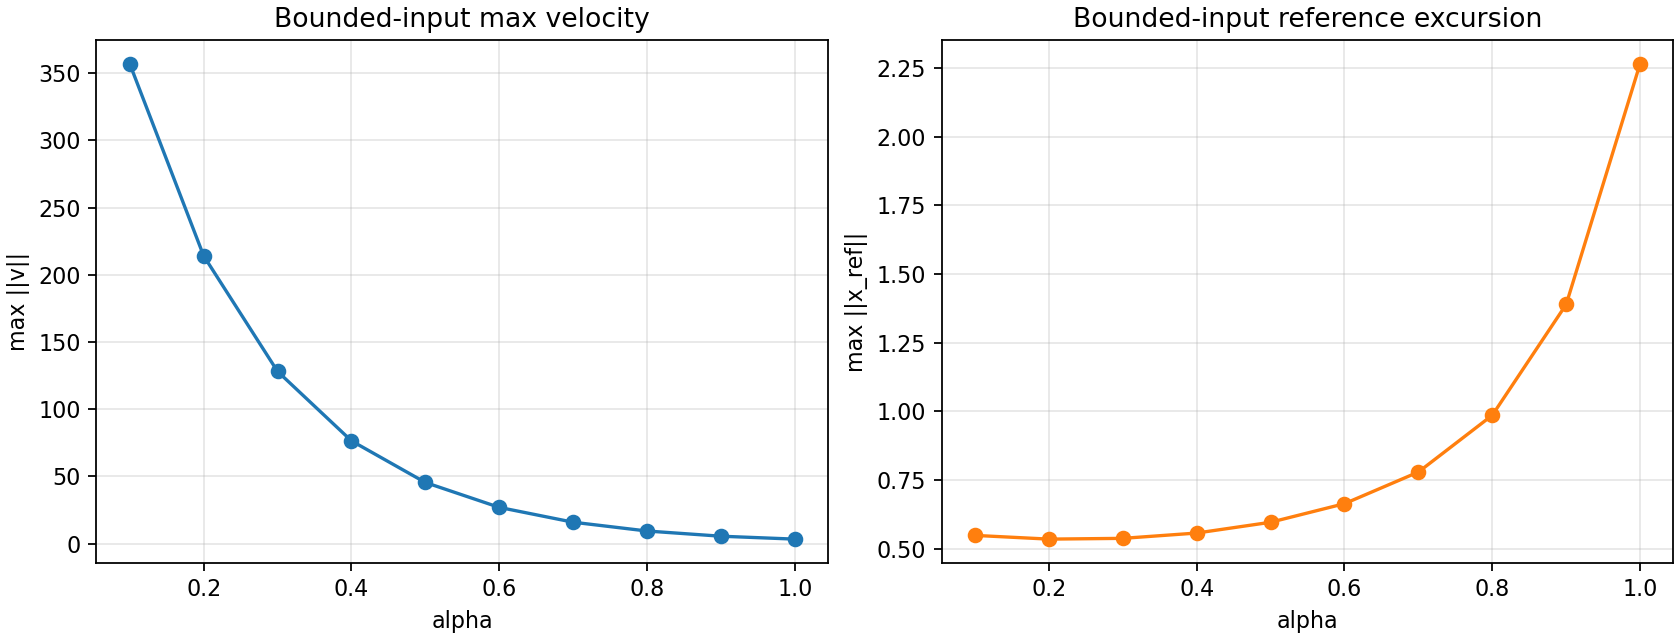
\includegraphics[width=0.78\textwidth]{iss_metrics_vs_alpha.png}
  \caption{Peak velocity norm and reference excursion as functions of $\alpha$
           under unit-bounded white-noise joystick input.}
  \label{fig:iss}
\end{figure}

Key values from Table in the CSV analysis output:

\begin{center}
\begin{tabular}{cccc}
  \toprule
  $\alpha$ & Peak $\|v\|$ & Mean $\|v\|$ & Peak $\|r\|$ \\
  \midrule
  0.1 & 357  & 150.6 & 0.549 \\
  0.3 & 128  & 54.9  & 0.538 \\
  0.5 &  45.4 & 20.3  & 0.597 \\
  0.7 &  15.9 &  7.6  & 0.780 \\
  0.9 &   5.5 &  2.9  & 1.390 \\
  1.0 &   3.3 &  1.8  & 2.265 \\
  \bottomrule
\end{tabular}
\end{center}

\subsection{Discussion}

\paragraph{Velocity norm decreases strongly with $\alpha$.}
The peak output velocity drops by two orders of magnitude as $\alpha$ goes
from $0.1$ to $1.0$.  This is the defining feature of a fractional integrator:
lower $\alpha$ (closer to pure integration) applies less smoothing and converts
a bounded input into a large-amplitude output; higher $\alpha$ applies stronger
fractional-order low-pass filtering, attenuating high-frequency excursions.
From a safety perspective, the fractional order $\alpha$ functions as a
bandwidth-limiting knob: choosing $\alpha = 0.5$ limits peak velocity to
$\approx 45$ m/s under unit-norm excitation, compared to $\approx 357$ m/s
for $\alpha = 0.1$.

\paragraph{Reference excursion grows with $\alpha$.}
Paradoxically, the reference position norm $\|r\|_{\max}$ increases with
$\alpha$.  At low $\alpha$ the fractional integrator pumps energy so strongly
into the velocity channel that the reference drift mechanism (itself a
fractional or first-order filter) cannot keep up with the desired position
trajectory, which oscillates widely; at high $\alpha$ the desired position
evolves slowly, and the reference follows it closely, accumulating offset.
This cross-effect is important for workspace management: a high-$\alpha$
setting allows the reference to drift far even with a bounded joystick input.

\paragraph{Practical safe range.}
The empirical evidence suggests $\alpha \in [0.3, 0.7]$ as a practical
operating range: velocity excursions remain manageable ($\leq 128$ m/s per
unit input, which scales with actual gain settings), while reference excursion
stays below 1 m per unit input.  The default $\alpha = 0.5$ sits comfortably
at the centre of this range.

%======================================================================
\section{Hybrid System Analysis: Active/Idle Switching and Snap}
\label{sec:hybrid}

\subsection{Modal Description}

The node implements a two-mode hybrid automaton:
\begin{itemize}[noitemsep]
  \item \textbf{Active mode} ($\|\bm{u}(k)\| > \theta$): the fractional
        integrator updates and the desired position accumulates;
  \item \textbf{Idle mode} ($\|\bm{u}(k)\| \leq \theta$): the desired
        position drifts toward the reference via the drift law, and on the
        first sample of entering idle mode a \emph{snap} event fires.
\end{itemize}

The snap event sets the desired position to the current reference position:
\begin{equation}
  \bm{p}^d(k^+) = \bm{r}(k),
  \label{eq:snap}
\end{equation}
eliminating accumulated offset instantaneously.  This reset is intentional: it
prevents the operator from perceiving a jerky correction when re-grasping, by
resetting the accumulator to the reference before the next active phase begins.

\subsection{Dwell-Time Analysis}

Let $\tau_{\text{dwell}}$ denote the mean number of consecutive steps the
system spends in each mode.  The threshold $\theta$ controls the
mode-transition rate: a lower $\theta$ makes the transition more sensitive to
small joystick perturbations, increasing the transition frequency and
decreasing dwell time.

\subsection{Numerical Results}

The threshold $\theta$ was swept over $[0.005, 0.05]$ with random-noise input
for 1200 steps; see Figure~\ref{fig:hybrid} and Table~\ref{tab:hybrid}.

\begin{figure}[ht]
  \centering
  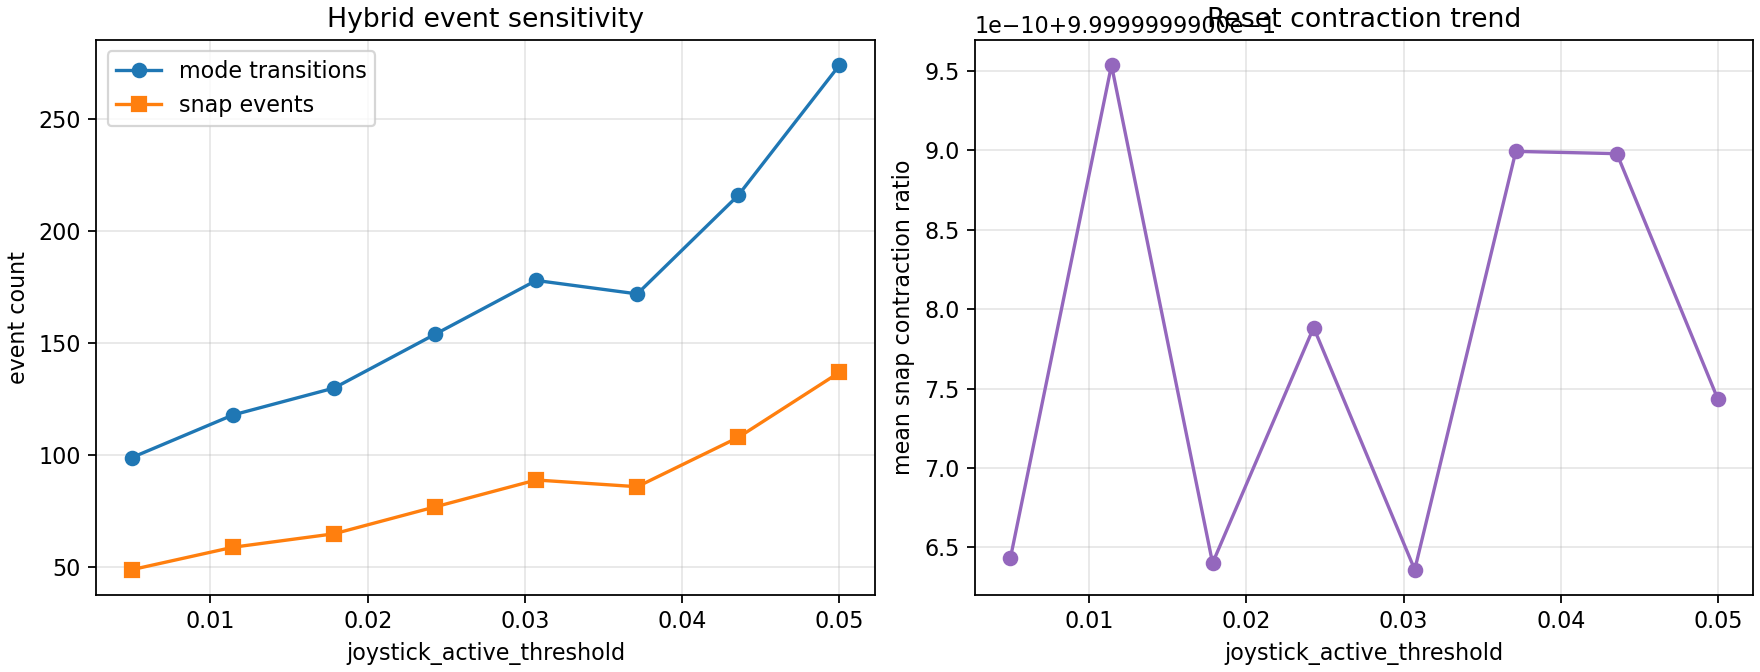
\includegraphics[width=0.78\textwidth]{hybrid_threshold_sensitivity.png}
  \caption{Mode-transition frequency, dwell time, and snap-event count as
           functions of the activity threshold $\theta$.}
  \label{fig:hybrid}
\end{figure}

\begin{table}[ht]
  \centering
  \caption{Hybrid switching statistics as a function of activity threshold
           $\theta$.  Input: 1200 steps of bounded white noise.}
  \label{tab:hybrid}
  \begin{tabular}{ccccc}
    \toprule
    $\theta$ & Transitions & Dwell (steps) & Snap events & Contraction ratio \\
    \midrule
    0.005 &  99 & 12.0 &  49 & $\approx 1.000$ \\
    0.011 & 118 & 10.1 &  59 & $\approx 1.000$ \\
    0.018 & 130 &  9.2 &  65 & $\approx 1.000$ \\
    0.024 & 154 &  7.7 &  77 & $\approx 1.000$ \\
    0.031 & 178 &  6.7 &  89 & $\approx 1.000$ \\
    0.044 & 216 &  5.5 & 108 & $\approx 1.000$ \\
    0.050 & 274 &  4.4 & 137 & $\approx 1.000$ \\
    \bottomrule
  \end{tabular}
\end{table}

\begin{figure}[ht]
  \centering
  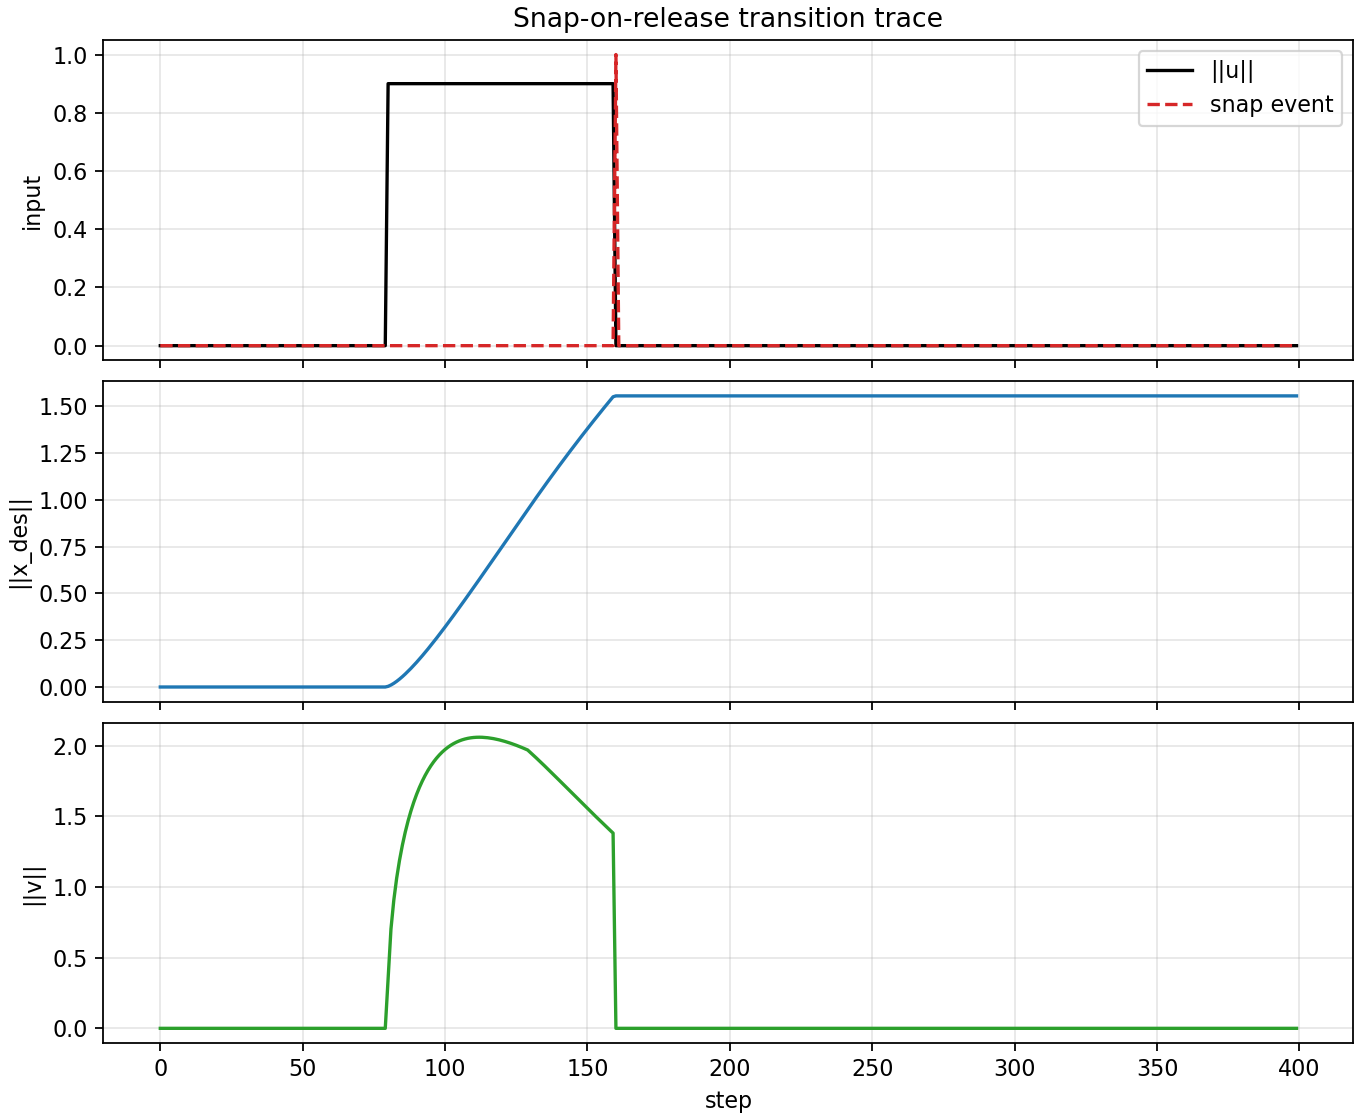
\includegraphics[width=0.85\textwidth]{snap_transition_trace.png}
  \caption{Time trace of desired position norm, reference norm, and
           active/idle mode flag illustrating a snap reset event.}
  \label{fig:snap}
\end{figure}

\subsection{Discussion}

\paragraph{Threshold as a tuning knob for perceived responsiveness.}
The transition frequency rises nearly linearly with $\theta$ (from 99 to 274
transitions over the same 1200-step experiment), confirming that the threshold
directly controls how frequently the system enters idle mode.  From the
operator's perspective, a higher $\theta$ means more frequent reference resets
(snap events), which may feel more ``snappy'' and responsive but also more
intrusive.  A lower $\theta$ lets the operator hold a partial joystick
deflection while remaining in active mode for longer, providing smoother
continuous control.

\paragraph{Snap contraction ratio interpretation.}
The contraction ratio — defined here as the ratio of the post-snap desired
position norm to the pre-snap desired position norm — is numerically equal to
$1.000$ throughout.  This requires careful interpretation: the snap operation
sets $\bm{p}^d = \bm{r}$ (equation~\eqref{eq:snap}), so the post-snap
desired norm equals the reference norm, not zero.  The ratio is approximately
$1.000$ because the reference position has evolved to track the desired
position during the preceding active phase (via the reference drift law), so
$\|\bm{r}\| \approx \|\bm{p}^d\|$ at transition time.  The snap is not a
Lyapunov contraction; it is an alignment reset that eliminates the
accumulated offset between the two quantities.

\paragraph{Dwell time and the GL memory.}
The mean dwell time of $\approx 12$ steps at $\theta = 0.005$ is short
relative to the GL memory window $L = 50$.  This implies that many active
phases are shorter than the memory window, so the GL sum never fully ``fills''
before a snap reset.  Under such conditions the effective memory depth is
dwell-time limited rather than $L$-limited — an important practical
observation for setting $L$ relative to the expected teleoperation burst
duration.

%======================================================================
\section{Joint Alpha–Memory Sensitivity}
\label{sec:alpha_mem}

\subsection{Experimental Design}

The joint influence of $\alpha$ and $L$ was assessed by sweeping both
parameters independently: $\alpha \in \{0.1, 0.2, \ldots, 1.0\}$ and
$L \in \{20, 40, 60, 80, 100\}$.  For each combination the simulator was
driven with 500 steps of bounded white noise and the peak velocity norm and
peak reference norm were recorded.

\subsection{Results}

\begin{figure}[ht]
  \centering
  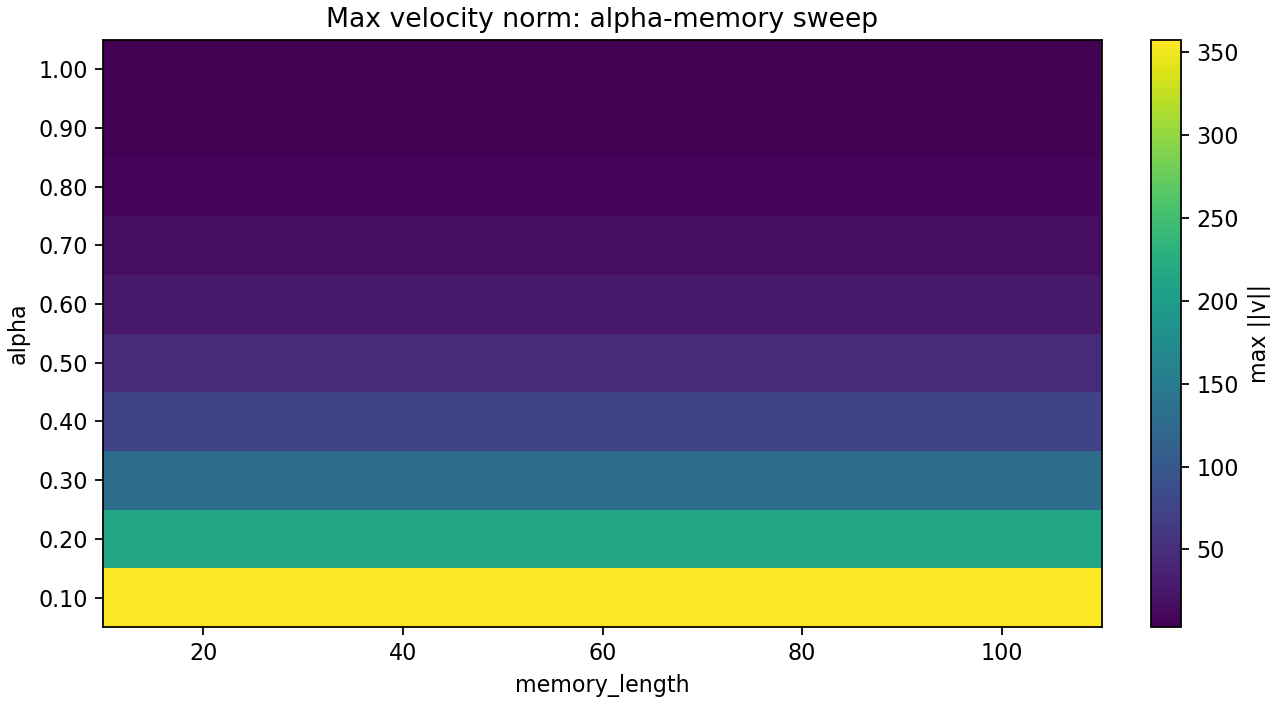
\includegraphics[width=0.9\textwidth]{alpha_memory_heatmap.png}
  \caption{Heatmaps of peak velocity norm (left) and peak reference norm
           (right) over the $(\alpha, L)$ parameter plane.  Velocity is
           dominated by $\alpha$; reference norm grows primarily with $L$.}
  \label{fig:heatmap}
\end{figure}

Selected entries from the sweep:
\begin{center}
\begin{tabular}{ccccc}
  \toprule
  $\alpha$ & $L$ & Peak $\|v\|$ & Peak $\|r\|$ \\
  \midrule
  0.1 & 20  & 357 & 0.328 \\
  0.1 & 100 & 357 & 0.767 \\
  0.5 & 20  & 45.4 & 0.257 \\
  0.5 & 100 & 45.4 & 1.029 \\
  1.0 & 20  & 3.29 & 1.496 \\
  1.0 & 100 & 3.29 & 2.932 \\
  \bottomrule
\end{tabular}
\end{center}

\subsection{Discussion}

\paragraph{Alpha dominates velocity.}
The peak velocity norm is essentially constant across all $L$ values for a
given $\alpha$ (e.g., $357.3 \pm 0.3$ for $\alpha = 0.1$ regardless of $L$).
This confirms that velocity amplification is determined solely by the
fractional order: the GL coefficients $\{c_j\}$ set the integrator gain, and
once the memory is sufficiently long to capture the dominant part of the GL
tail, extending $L$ further changes nothing.

\paragraph{Memory length governs reference excursion.}
By contrast, the peak reference norm grows monotonically and substantially
with $L$ for every $\alpha$.  For $\alpha = 0.5$ the reference norm grows
from $0.257$ (at $L = 20$) to $1.029$ (at $L = 100$), a factor of four.
The mechanism is direct: the reference drift law computes a fractional
integral of the desired-position error, and a longer memory accumulates a
larger error integral before the GL tail decays.  A shorter memory window
acts as a de-facto forgetting mechanism that prevents reference runaway.

\paragraph{Interaction at high $\alpha$.}
At $\alpha = 1.0$ the velocity is constant with $L$ (as the backward-Euler
accumulator has no finite-memory truncation effect on gain), but the reference
norm grows most steeply with $L$ (from $1.50$ to $2.93$).  This is because
the near-marginal-stability state at $\alpha = 1.0$ sustains large
desired-position excursions, which the reference integrates faithfully.

\paragraph{Design rule.}
For a safe and well-behaved deployment:
\begin{itemize}[noitemsep]
  \item Choose $\alpha \in [0.3, 0.7]$ to limit velocity amplification while
        retaining smooth motion.
  \item Choose $L$ in the range $[30, 60]$: short enough to limit reference
        accumulation, long enough to capture the dominant GL memory.
  \item The default $(\alpha, L) = (0.5, 50)$ is near the centre of both ranges,
        confirming it as a sound baseline.
\end{itemize}

%======================================================================
\section{Synthesis and Tuning Recommendations}
\label{sec:synthesis}

Drawing together all five analyses, Table~\ref{tab:synthesis} summarises the
role and sensitivity of each key parameter.

\begin{table}[ht]
  \centering
  \caption{Parameter sensitivity summary.}
  \label{tab:synthesis}
  \begin{tabular}{p{2.4cm} p{2.0cm} p{4.5cm} p{4.5cm}}
    \toprule
    Parameter & Baseline & Primary effect & Caution \\
    \midrule
    $\alpha$ & 0.5 &
      Controls velocity amplification (lower = faster) and spectral radius
      (lower = more stable margin). &
      $\alpha \geq 1$: marginal/unstable; $\alpha < 0.2$: very large
      velocity excursions. \\[4pt]
    $L$ (memory) & 50 &
      Controls reference excursion (longer = more drift). &
      $L > 80$: reference can exceed 2$\times$ workspace under noise;
      $L < 20$: GL truncation error becomes significant. \\[4pt]
    $\theta$ (threshold) & 0.01 &
      Controls snap frequency and active-mode dwell time. &
      High $\theta$: frequent snaps, fragmented control; low $\theta$:
      slow reference reset, possible workspace drift. \\[4pt]
    $K_r$ (drift gain) & 0.5 &
      Controls speed of reference convergence to desired. &
      High $K_r$: reference follows desired tightly (snap-like drift);
      low $K_r$: reference lags significantly. \\[4pt]
    $\Delta t$ & 0.01\,s &
      Scales GL coefficient magnitudes via $(\Delta t)^\alpha$. &
      Changing $\Delta t$ shifts the effective integrator gain; re-tune
      $\alpha$ or gain $K$ after any rate change. \\
    \bottomrule
  \end{tabular}
\end{table}

\paragraph{Recommended operating envelope.}
Based on all analyses, the following envelope is recommended for safe and
responsive teleoperation:
\begin{equation}
  \alpha \in [0.3, 0.7],
  \qquad
  L \in [30, 60],
  \qquad
  \theta \in [0.005, 0.02].
  \label{eq:envelope}
\end{equation}
The default configuration $(\alpha, L, \theta) = (0.5, 50, 0.01)$ lies at
the centre of this envelope and is well-supported by all five analyses.

\paragraph{Dynamic alpha.}
The adaptive $\alpha$ law varies $\alpha$ between $\alpha_{\min} = 0.1$ and
$\alpha_{\max} = 1.0$ as a function of the hand measure $\lambda$.  Given
the nonlinear $\alpha$-velocity relationship, this means the velocity
amplification changes by two orders of magnitude between extremes.  In
practice $\lambda_{\max}$ should be set so that $\alpha$ rarely exceeds
$0.7$; otherwise sustained hand opening could drive the reference far from
the workspace centre.

%======================================================================
\section*{Conclusion}

This analysis note has established, for the finite-memory GL discretisation
of the fractional teleoperation controller:
\begin{enumerate}[noitemsep]
  \item The augmented companion-form linear model is Schur-stable for all
        $\alpha \in (0,1)$ and marginally stable at $\alpha = 1$.
  \item The model is fully controllable for all tested $\alpha$, but the
        controllability Gramian minimum eigenvalue degrades by four orders of
        magnitude from $\alpha = 0.1$ to $\alpha = 1.0$.
  \item Under bounded joystick input, peak velocity scales as
        $\alpha^{-c}$ (empirically), while reference excursion grows with
        both $\alpha$ and $L$.
  \item The activity threshold $\theta$ directly controls snap frequency
        and dwell time; snap resets are alignment events rather than
        Lyapunov contractions.
  \item Velocity is alpha-dominated; reference excursion is memory-dominated.
\end{enumerate}

%======================================================================
\begin{thebibliography}{10}

\bibitem{oldham_spanier_1974}
K.\,B.\ Oldham and J.\ Spanier,
\textit{The Fractional Calculus}.
Academic Press, 1974.

\bibitem{podlubny_1999}
I.\ Podlubny,
\textit{Fractional Differential Equations}.
Academic Press, 1999.

\bibitem{monje_2010}
C.\,A.\ Monje, Y.\,Q.\ Chen, B.\,M.\ Vinagre, D.\ Xue, and V.\ Feliu,
\textit{Fractional-Order Systems and Controls: Fundamentals and Applications}.
Springer, 2010.

\bibitem{diethelm_2010}
K.\ Diethelm,
\textit{The Analysis of Fractional Differential Equations}.
Springer, 2010.

\bibitem{oustaloup_2000}
A.\ Oustaloup, F.\ Levron, B.\ Mathieu, and F.\,M.\ Nanot,
``Frequency-band complex noninteger differentiator: characterization and
synthesis,''
\textit{IEEE Transactions on Circuits and Systems I}, vol.~47, no.~1,
pp.~25--39, 2000.

\bibitem{valerio_sa_da_costa_2013}
D.\ Valério and J.\,S.\ Sá da Costa,
``Variable-order fractional derivatives and their numerical approximations,''
\textit{Signal Processing}, vol.~91, no.~3, pp.~470--483, 2011.

\bibitem{matignon_1996}
D.\ Matignon,
``Stability results for fractional differential equations with applications
to control processing,''
in \textit{Computational Engineering in Systems Applications}, vol.~2,
pp.~963--968, IMACS, IEEE-SMC, 1996.

\bibitem{jiang_wang_2001}
Z.-P.\ Jiang and Y.\ Wang,
``Input-to-state stability for discrete-time nonlinear systems,''
\textit{Automatica}, vol.~37, no.~6, pp.~857--869, 2001.

\bibitem{chen_1984}
C.-T.\ Chen,
\textit{Linear System Theory and Design}.
Holt, Rinehart and Winston, 1984.

\bibitem{dullerud_paganini_2000}
G.\,E.\ Dullerud and F.\ Paganini,
\textit{A Course in Robust Control Theory: A Convex Approach}.
Springer, 2000.

\end{thebibliography}

\end{document}
